The  LT3741  is both  voltage  regulated  and current  regulated. The  voltage
divider  $R_{11} \parallel  R_2$  (see figure  \ref{fig:circuit:buck} on  page
\pageref{fig:circuit:buck}  and  figure  \ref{fig:circuit:buck:uset}  on  page
\pageref{fig:circuit:buck:uset})  allows for  the  measurement  of the  output
voltage, and  a shunt resistor  $R_4$ allows for  the exact monitoring  of the
current going through  coil $L_1$. The value for resistor $R_4$  was chosen so
that the maximum outoing current can be \SI{5}{\ampere}.

\begin{figure}[th!]
    \center
    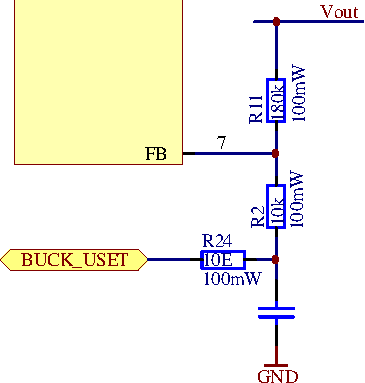
\includegraphics[width=.35\textwidth]{images/circuit/buck-uset.pdf}
    \caption{regulation of output voltage by changing the reference voltage in the feedback loop via an analog reference voltage between \SI{0}{\volt} and \SI{1.21}{\volt}}
    \label{fig:circuit:buck:uset}
\end{figure}

Monitoring  the current  is  extremely  important for  a  setup  in which  the
outgoing  voltage can  be constantly  changing. It allows  to more  accurately
predict the behavior of the output voltage, thus enabling the device to better
suppress spikes in output voltage and spikes in the current going through coil
$L_1$. % TODO: correct coil?

Furthermore, a controller regulated by current  can also be used as a constant
current source. This property is mainly of importance when the operating point
is in  the steeper part  of the PV module's  I-V-curve (where small  changes in
voltage can lead to drastic changes in current and vice versa).

The values for the feedback resistors $R_2$ and $R_{11}$ were chosen according
to formula \ref{eq:circuit:buck:feedback_resistors} so that the output voltage
does not exceed \SI{23}{\volt}:

\begin{equation}
    V_{out} = \SI{1.21}{\volt} \left( 1 + \frac{R_{11}}{R_2} \right)
    \label{eq:circuit:buck:feedback_resistors}
\end{equation}

By increasing $BUCK\_USET$ in formula \ref{eq:circuit:buck:uset}, the outgoing
voltage can then be modified as needed:

\begin{equation}
    V_{out} = (\SI{1.21}{\volt} - BUCK\_USET) \cdot \frac{R_{11} + R_2}{R_2}
    \label{eq:circuit:buck:uset}
\end{equation}

$BUCK\_USET$ is the  analog voltage coming from the  first DAC. The associated
circuit can be found in figure \ref{fig:circuit:buck:uset}.

In a  manner analogous to  regulating the  output voltage, the  maximum output
current  can  also be  controlled.   By  applying  an analog  voltage  between
\SI{0}{\volt}  and  \SI{1.5}{\volt}  at   input  \code{CTRL1}  of  the  LT3741
controller, the  maximum \emph{average} current  going through coil  $L_1$ and
therefore the maximum output current can be directly controlled.

\begin{figure}[th!]
    \center
    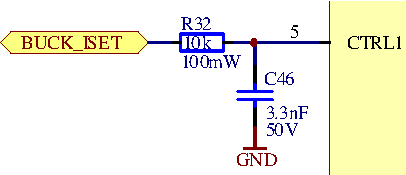
\includegraphics[width=.4\textwidth]{images/circuit/buck-iset.pdf}
    \caption{Setting the maximum output current via reference voltage between \SI{0}{\volt} and \SI{1.5}{\volt}}
    \label{fig:circuit:buck:iset}
\end{figure}

The corresponding circuit can be  found in figure \ref{fig:circuit:buck:iset}.
The maximum  average   output  current  $I_o$  is   calculated  using  formula
\ref{eq:circuit:buck:output_current}.

\begin{equation}
    I_o = \frac{V_{CTRL1}}{30 \cdot R_4}
    \label{eq:circuit:buck:output_current}
\end{equation}

For this, $V_{CTRL1}$  is the analog reference voltage coming  from the second
DAC and  $R_4$ is the  shunt resistor (\SI{10}{\milli\ohm}, visible  in figure
\ref{fig:circuit:buck}).

For the microcontroller  to generate appropriate reference  voltages, it needs
to  measure both  output voltage  and  output current. The  output voltage  is
measured with  the circuit in figure  \ref{fig:circuit:buck:umeas}. The values
for resistors  $R_{12}$ and  $R_{15}$ are such  that voltage  $BUCK\_UMEAS$ is
scaled to the range between \SI{0}{\volt} and \SI{1.5}{\volt}.

\begin{figure}[th!]
    \center
    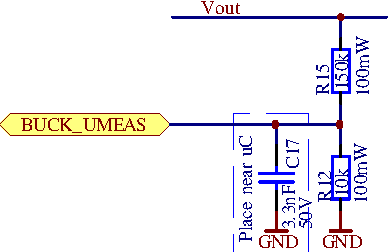
\includegraphics[width=.45\textwidth]{images/circuit/buck-umeas.pdf}
    \caption{Messen der Ausgangsspannung}
    \label{fig:circuit:buck:umeas}
\end{figure}

The output  current is measured  differentially via shunt  resistor $R_5$. The
corresponding circuit can be seeen in figure \ref{fig:circuit:buck:imeas}.

\begin{figure}[th!]
    \center
    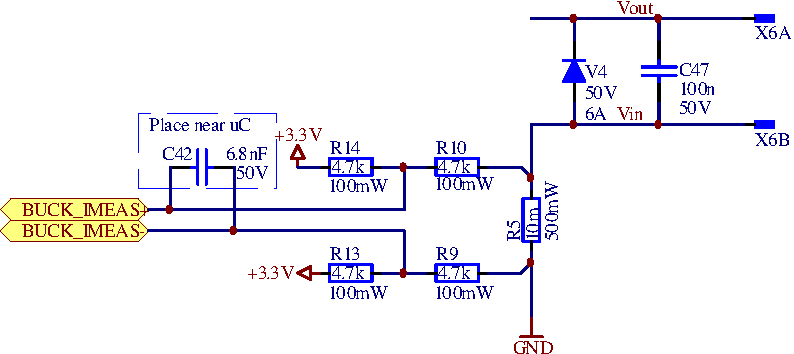
\includegraphics[width=.85\textwidth]{images/circuit/buck-imeas.pdf}
    \caption{Messen des Ausgangsstromes}
    \label{fig:circuit:buck:imeas}
\end{figure}

A  particular problem  for this  measurement  is that  resistors $R_{10}$  and
$R_{14}$ cause a  bias current to flow through the  shunt resistor $R_5$, thus
leading to an offset $V_{offset}$ of the measured voltage over $R_5$:

\begin{equation}
    V_{offset} = \frac{ \SI{3.3}{\volt} \cdot R_5 }{ R_{14} + R_{10} + R_5 }
    \label{eq:circuit:buck:shunt_offset}
\end{equation}

Since  the  ADC has  a  resolution  of 12  bits  and  a reference  voltage  of
\SI{3.3}{\volt},  one voltage  increment can  be calcualted  according to  the
following equation:

\begin{equation}
    V_{step} = \frac{\SI{3.3}{\volt}}{2^{12}} = \SI{806}{\micro\volt}
    \label{eq:circuit:buck:adc_step}
\end{equation}

Resistors  $R_9$, $R_{10}$, $R_{10}$ and  $R_{14}$  should be as small as possible%TODO: 2 times R10
in order to  reduce disturbances in the  traces, while at the  same time being
large enough for $V_{offset}$ to be  smaller than $V_{step}$. In order for the
ADC's  holding  time not  to  be  too long  (which  happens  roughly at  $\geq      %TODO What is smaller or equal than 5kohm?
\SI{5}{\kilo\ohm}$), they should however also not be too large.

Equations \ref{eq:circuit:buck:shunt_offset} \ref{eq:circuit:buck:adc_step} can now
be solved for the four resistor values:

\begin{align*}
                          V_{step} &\geq V_{offset} \\
    \frac{\SI{3.3}{\volt}}{2^{12}} &\geq \SI{3.3}{\volt} \cdot \frac{R_5}{R_x + R_5} \\
                  \frac{1}{2^{12}} &\geq \frac{R_5}{R_x + R_5} \\
                               R_x &\geq \left( 2^{12} - 1 \right) \cdot R_5 \\
\end{align*}

where $\frac{R_x}{2} =  R_{9} = R_{10} = R_{13} =  R_{14}$. This yields as its
result $\frac{R_x}{2} \approx \SI{22}{\ohm}$.

A further limitation, especially for smaller resistors, is not to dissipate too much
power. For this reason, the resistors will be dimensioned slightly higher at % TODO: slightly higher: 270 vs 22 ohm?
\SI{270}{\ohm}. Thus, the  resulting dissipated  power for  all
four resistors comes to:

\begin{equation*}
    P_{loss} \approx \frac{\left(\SI{3.3}{\volt}\right)^2}{2\cdot \SI{270}{\ohm}} \approx \SI{20}{\milli\watt}
\end{equation*}

The measured  voltage at the  shunt resistor is comparatively  small. For this reason,
we use the microcontroller's integrated preamplifier (PGA), %TODO correct term for Vorverstaerker?
which can  attain a  gain of  up to  factor 64. The  amplified signal  is then
passed on to the internal differential ADC.
